\documentclass[12pt]{article} % use larger type; default would be 10pt
\usepackage[czech]{babel}
\usepackage[utf8]{inputenc} % set input encoding (not needed with XeLaTeX)

%%% PAGE DIMENSIONS
\usepackage{geometry} % to change the page dimensions
% \usepackage[left=2cm,right=2cm,top=2cm,bottom=2cm]{geometry}
\geometry{a4paper}
% \geometry{margin=2in} % for example, change the margins to 2 inches all round
% \geometry{landscape} % set up the page for landscape

\usepackage{graphicx} % support the \includegraphics command and options
\usepackage{wrapfig} % support the wrapfigure section

\usepackage{hyperref} % links in \tableofcontents
\hypersetup{
	colorlinks,
	citecolor=black,
	filecolor=black,
	linkcolor=black,
	urlcolor=black
}

% \usepackage[parfill]{parskip} % Activate to begin paragraphs with an empty line rather than an indent

%%% PACKAGES
\usepackage{booktabs} % for much better looking tables
\usepackage{array} % for better arrays (eg matrices) in maths
%\usepackage{paralist} % very flexible & customisable lists (eg. enumerate/itemize, etc.)
\usepackage{verbatim} % adds environment for commenting out blocks of text & for better verbatim
\usepackage{subfig} % make it possible to include more than one captioned figure/table in a single float
% These packages are all incorporated in the memoir class to one degree or another...
\usepackage{tikz} % graphs
\usepackage{pgfplots}
\usepackage{float}

%%% HEADERS & FOOTERS
\usepackage{fancyhdr} % This should be set AFTER setting up the page geometry
\pagestyle{fancy} % options: empty , plain , fancy
\renewcommand{\headrulewidth}{0pt} % customise the layout...
\lhead{}\chead{}\rhead{}
\lfoot{}\cfoot{\thepage}\rfoot{}

%%% SECTION TITLE APPEARANCE
\usepackage{sectsty}
\allsectionsfont{\sffamily\mdseries\upshape} % (See the fntguide.pdf for font help)
% (This matches ConTeXt defaults)

%%% ToC (table of contents) APPEARANCE
\usepackage[nottoc,notlof,notlot]{tocbibind} % Put the bibliography in the ToC
\usepackage[titles,subfigure]{tocloft} % Alter the style of the Table of Contents
\renewcommand{\cftsecfont}{\rmfamily\mdseries\upshape}
\renewcommand{\cftsecpagefont}{\rmfamily\mdseries\upshape} % No bold!
\newcommand{\bigsize}{\fontsize{35pt}{20pt}\selectfont}

%%% END Article customizations

\begin{document}
\begin{titlepage}
	
\includegraphics[scale=0.7]{logo.jpg}
	\vspace*{\fill}
	\begin{center}
		\textsc{\LARGE Katedra technologií a měření}\\[0.3cm]
		\textsc{\LARGE \bigsize Fyzikální elektronika}\\[0.3cm]
		\textsc{\LARGE Měření statických charakteristik diod}\\[1cm]
		Martin Zlámal \\[1cm]
		{\small\em \ Datum měření 7. října 2013 } \\
		{\small\em \copyright \ Datum poslední revize \today } \\
		\LaTeX
	\end{center}
	\vspace*{\fill}
\end{titlepage}
\tableofcontents
\listoffigures
\listoftables
\newpage

\section{Zadání}
\begin{enumerate}
\item Vyhledejte v katalogu pro každou z předložených diod mezní hodnoty
propustného proudu $I_F$ (F z angl. "forward") a závěrného napětí $U_R$ (R z
angl. "reverse") a poznamenejte si je.
\item Navrhněte schémata pro měření voltampérové charakteristiky diod
v propustném a závěrném směru (nestačí pouze otočit polaritu napětí na
diodě). V zapojení použijte ochranný odpor o hodnotě $1k\Omega$.
\item Změřte V-A charakteristiky pro zadané typy polovodičových diod v
propustném i závěrném směru. Diody LED měřte pouze v propustném směru
a maximálně do $\mathbf{15 mA}$.
\item Ve zvoleném pracovním bodě stanovte statický a dynamický odpor diod.
\item Najděte analytickou funkci, která aproximuje charakteristiku diody,
vycházejte ze Shockleyho rovnice. Zvolte si jednu diodu a tuto funkci vyneste
do samostatného grafu.
\item Naměřené V-A charakteristiky vyneste do grafů. Propustný směr všech diod
bude umístěn do jednoho grafu. Totéž platí pro závěrný směr. Dbejte na
správné umístění charakteristik do příslušných kvadrantů osového kříže.
\item Do závěru porovnejte prahové napětí změřených diod a určete typ diody (Si,
Ge a Shotkyho). Porovnejte a zhodnoťte statické a dynamické odpory diod.
\end{enumerate}

\section{Schéma zapojení}
\begin{figure}[H]
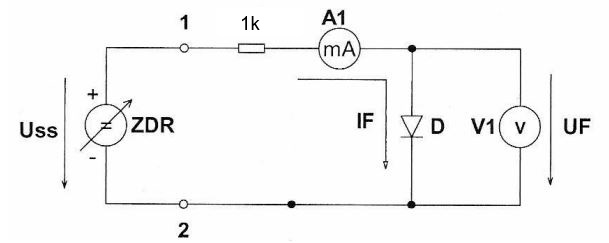
\includegraphics[scale=1]{propustny.jpg}
\caption{Schéma pro měření V-A charakteristiky v propustném směru}
\end{figure}

\begin{figure}[H]
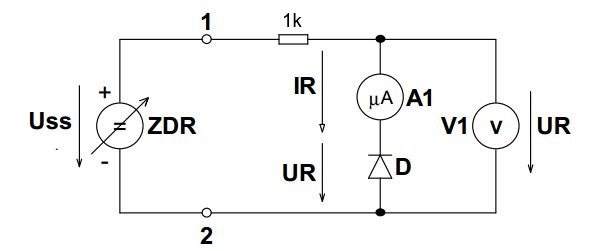
\includegraphics[scale=1]{zaverny.jpg}
\caption{Schéma pro měření V-A charakteristiky v závěrném směru}
\end{figure}
\newpage

\section{Naměřené a vypočtené hodnoty}
\subsection{Mezní katalogové parametry součástek}
\captionof{table}{Mezní katalogové parametry diod}
\begin{tabular}{|c|c|c|}
\hline 
Typ diody & Mezní hodn. prop. proudu $I_F$ & Mezní hodn. závěr. napětí $U_R [V]$ \\ 
\hline 
Modrá LED & 20mA & 3V \\ 
\hline 
Žlutá LED & 20mA & 2,1V \\ 
\hline 
1N4007 & 1A & 1000V \\ 
\hline 
D9D & 50mA & 30V \\ 
\hline 
SB 360 & 3A & 60V \\ 
\hline 
KY 130/150 & 30mA & 180V \\ 
\hline 
\end{tabular}

\subsection{Výpočet statického odporu diod}
Statický odpor vypočítávám ze zvoleného pracovního bodu viz zadání s využitím ohmova zákona:
\begin{equation}
R_{S(BlueLED)}=\frac{U}{I}=\frac{3,56}{4,39\cdot 10^{-3}}=810,934\Omega
\end{equation}
\begin{equation}
R_{S(YellowLED)}=\frac{U}{I}=\frac{2,35}{5,97\cdot 10^{-3}}=393,635\Omega
\end{equation}
\begin{equation}
R_{S(1N4007)}=\frac{U}{I}=\frac{0,66}{9,3\cdot 10^{-3}}=70,9677\Omega
\end{equation}
\begin{equation}
R_{S(D9D)}=\frac{U}{I}=\frac{0,34}{8,5\cdot 10^{-3}}=40,0\Omega
\end{equation}
\begin{equation}
R_{S(SB 360)}=\frac{U}{I}=\frac{0,19}{7,7\cdot 10^{-3}}=24,6753\Omega
\end{equation}
\begin{equation}
R_{S(KY 130/150)}=\frac{U}{I}=\frac{0,62}{137,778\cdot 10^{-3}}=24,6753\Omega
\end{equation}

\subsection{Výpočet dynamického odporu diod}
Dynamický (diferenciální) odpor vypočítávám ze zvoleného pracovního bodu viz zadání s využitím ohmova zákona. Používám hodnoty blízké k hodnotám při výpočtu statického odporu diod. Dynamický odpor se mění v závislosti na tom, kde na křivce zvolíme pracovní bod.

Pro výpočet dynamického odporu je zapotřebí znát směrnici tečny funkce v konkrétním bodě což je vlastně:
\begin{equation}
r_D=\frac{dU}{dI}
\end{equation}
Pro derivaci bych však musel znát přesný předpis funkce, což v tomto případě není možné, jelikož výstupem měření jsou pouze body. Pro skutečné měření se proto používá spíše rovnice:
\begin{equation}
r_D=\frac{\Delta U}{\Delta I}
\end{equation}
Pokud se budu limitně blížit proudem k nule, získám teoretický derivační vztah. Výpočet se tedy provádí tak, že změříme proud, který protéká diodou při daném napětí. Poté zvětšíme protékaný proud a opět obě hodnoty odečteme.\footnote{doc. Ing. Július Štelina, CSc. - Meranie dynamického odporu polovodičových diód}  Tím můžeme využít onoho rozdílového vtahu. Tento postup bude tím přesnější, čím bude $\Delta U$ resp. $\Delta I$ menší.
\begin{equation}
r_{D(BlueLED)}=\frac{\Delta U}{\Delta I}=\frac{U_2-U_1}{I_2-I_1}=\frac{3,56-3,46}{4,39\cdot 10^{-3}-2,49\cdot 10^{-3}}=52,6316\Omega
\end{equation}
\begin{equation}
r_{D(YellowLED)}=\frac{\Delta U}{\Delta I}=\frac{U_2-U_1}{I_2-I_1}=\frac{2,35-2,22}{5,97\cdot 10^{-3}-3,92\cdot 10^{-3}}=63,4146\Omega
\end{equation}
\begin{equation}
r_{D(1N4007)}=\frac{\Delta U}{\Delta I}=\frac{U_2-U_1}{I_2-I_1}=\frac{0,66-0,65}{9,3\cdot 10^{-3}-7,2\cdot 10^{-3}}=4,7619\Omega
\end{equation}
\begin{equation}
r_{D(D9D)}=\frac{\Delta U}{\Delta I}=\frac{U_2-U_1}{I_2-I_1}=\frac{0,34-0,33}{8,5\cdot 10^{-3}-7,0\cdot 10^{-3}}=6,6667\Omega
\end{equation}
\begin{equation}
r_{D(SB 360)}=\frac{\Delta U}{\Delta I}=\frac{U_2-U_1}{I_2-I_1}=\frac{0,19-0,18}{7,7\cdot 10^{-3}-6,1\cdot 10^{-3}}=6,2500\Omega
\end{equation}
\begin{equation}
r_{D(KY 130/150)}=\frac{\Delta U}{\Delta I}=\frac{U_2-U_1}{I_2-I_1}=\frac{0,62-0,61}{4,5\cdot 10^{-3}-3,3\cdot 10^{-3}}=8,3333\Omega
\end{equation}

\section{Grafy}
\begin{figure}[H]
\centering
	\begin{tikzpicture}
		\begin{axis}[
			width=1\textwidth,
	      	height=0.5\textwidth,
			xlabel={$U[V]$},
			ylabel={$I[mA]$}]
			
		\addplot coordinates {
			(0,0)
			(3.02,0.11)
			(3.20,0.35)
			(3.33,0.95)
			(3.46,2.49)
			(3.56,4.39)
			(3.70,7.54)
			(3.78,9.62)
			(3.87,12.15)
			(3.97,15)
		};
		\addlegendentry{Modrá LED}
		
		\addplot coordinates {
			(0,0)
			(1.74,0.18)
			(1.93,0.95)
			(2.11,2.45)
			(2.22,3.92)
			(2.35,5.97)
			(2.51,9.65)
			(2.60,11.88)
			(2.67,13.96)
			(2.71,14.92)
		};
		\addlegendentry{Žlutá LED}
		
		\addplot coordinates {
			(0,0)
			(0.54,0.5)
			(0.61,2.8)
			(0.64,5.4)
			(0.65,7.2)
			(0.66,9.3)
			(0.67,11.4)
			(0.68,13.6)
			(0.69,16.1)
			%(0.70,20)
		};
		\addlegendentry{1N4007}
		
		\addplot coordinates {
			(0,0)
			(0.21,0.8)
			(0.29,3.5)
			(0.32,5.4)
			(0.33,7.0)
			(0.34,8.5)
			(0.36,11.2)
			(0.38,14.2)
			(0.40,17.4)
			%(0.41,19.9)
		};
		\addlegendentry{D9D}
		
		\addplot coordinates {
			(0,0)
			(0.15,1.7)
			(0.15,2.1)
			(0.17,4.2)
			(0.18,6.1)
			(0.19,7.7)
			(0.19,8.6)
			(0.19,10.2)
			(0.20,12.2)
			(0.21,15.1)
		};
		\addlegendentry{SB 360}
		
		\addplot coordinates {
			(0,0)
			(0.56,1.1)
			(0.59,2.1)
			(0.61,3.3)
			(0.62,3.9)
			(0.62,4.5)
			(0.64,6.7)
			(0.66,8.8)
			(0.67,10.8)
			(0.67,13.0)
		};
		\addlegendentry{KY 130/150}
		
		\end{axis}
	\end{tikzpicture}
	\caption{V-A charakteristika - propustný směr}
\end{figure}

\begin{figure}[H]
\centering
	\begin{tikzpicture}
		\begin{axis}[
			width=1\textwidth,
	      	height=0.5\textwidth,
			xlabel={$U[V]$},
			ylabel={$I[uA]$},
			legend style={
				at={(0.73,0.05)},
				anchor=south west
			}
		]
		
		\addplot coordinates {
			(0,0)
			(-20,0)
		};
		\addlegendentry{1N4007}
		
		\addplot coordinates {
			(0,0)
			(-1.1,-3)
			(-3.5,-4)
			(-5.5,-4.7)
			(-6.5,-5.1)
			(-8.5,-5.9)
			(-10.1,-6.4)
			(-11.0,-6.7)
			(-13.8,-7.8)
			(-15.5,-8.5)
			(-17.5,-9.5)
			(-20,-10.6)
		};
		\addlegendentry{D9D}
		
		\addplot coordinates {
			(0,0)
			(-0.5,-6.9)
			(-1.0,-7.7)
			(-3.4,-10.5)
			(-5.8,-13.2)
			(-8.1,-15.3)
			(-10.4,-17.6)
			(-13.5,-20.7)
			(-15.2,-22.5)
			(-18.3,-25.7)
			(-20.3,-27.9)
		};
		\addlegendentry{SB 360}
		
		\addplot coordinates {
			(0,0)
			(-19,0)
		};
		\addlegendentry{KY 130/150}
		
		\end{axis}
	\end{tikzpicture}
	\caption{V-A charakteristika - závěrný směr}
\end{figure}

\begin{figure}[H]
\centering
	\begin{tikzpicture}[domain=0:4]
   		\begin{axis}[
			width=1\textwidth,
	      	height=0.5\textwidth,
			xlabel={$U[V]$},
			ylabel={$I[uA]$},
			legend style={
				at={(0.02,0.95)},
				anchor=north west
			}
		]
    	\addplot coordinates {
			(0,0)
			(3.02,0.11)
			(3.20,0.35)
			(3.33,0.95)
			(3.46,2.49)
			(3.56,4.39)
			(3.70,7.54)
			(3.78,9.62)
			(3.87,12.15)
			(3.97,15)
		};
		\addlegendentry{Modrá LED}
   		\addplot[color=red] {(20.6131/(1+(2.2383*10^9)*(e^(-5.67475*x))))-0.183578};
   		\addlegendentry{Logistická regrese}
   		\addplot[color=green] {0.00006*(20.7061)^x};
    	\addlegendentry{Exponenciální regrese}
    \end{axis}
	\end{tikzpicture}
	\caption{V-A charakteristika - regrese průběhu LED diody}
\end{figure}

V-A charakteristika modré LED diody je aproximována logistickou regresí, konkrétně se jedná o následující funkci:
\begin{equation}
y=\frac{20.6131}{1+2.2383\cdot 10^9 \cdot e^{-5.67475\cdot x}}-0.183578
\end{equation}
Tím získáme poměrně velmi přesnou aproximaci naměřených hodnot. Jednodušší avšak méně přesnou aproximaci naměřených hodnot získáme exponenciální regresí:
\begin{equation}
y=0.00006\cdot (20.7061)^x
\end{equation}
Tato aproximace je na jednu stranu nepřesná v měřeném úseku, na druhou stranu je snadno předvídatelnná. Logisitcká regrese oproti exponenciální velmi dobře aproximuje konkrétní měřené hodnoty, avšak mimo definiční obor a měřený obor hodnot již nabývá nesprávných hodnot.

\section{Závěr}
Celkem bylo měřeno šest druhů diod. Dvě svítivé LED (modrá a žlutá), dále dvě usměrňovací (1N4007 a KY 130/150), germaniová (D9D) a Schottkyho dioda (SB 360). Za povšimnutí stojí, že usměrňovací diody, ačkoliv jsou odlišné, mají velice podobné V-A charakteristiky.

Prahová napětí se v rozsahu měření velmi liší. Největší hodnotu prahového napětí naměříme na svítivých LED diodách, konkrétně na modré viz graf V-A charakteristika v propustném směru. Usměrňovací diody mají prahové napětí stejné a to přibližně $0,5V$. Nejmenší prahová napětí naměříme na Schottkyho diodě a o něco málo větší na germaniové diodě.

\end{document}
